\newpage
\chapter{Results}
\label{experiment_results}
\lhead{\emph{Experimental Results}}
We first present a full replication and extension of the work by
\citet{radDeliberationSinglePeakednessCoherent2021}. Then we present the simulations based on our model of
meta-deliberation, as well as the results of the sensitivity analysis on both
models. All code for the replication, main experiment and visualizations can be
found in \href{https://github.com/amirsahrani/master_thesis}{this Repository}. \Cref{AppendixB} contains all the values and ranges used for the experiments, as well as supplementary figures.


\section{Replication} We are able to fully replicate the results found by
\citet{radDeliberationSinglePeakednessCoherent2021},  in \Cref{fig:rep_cyclic}
we see that while the bias is less than 0.73, all metric results in a-cyclic
preferences. We also replicate the behavior of the KS metric, where biases in
the range of 0.73-0.85, show even some initial a-cyclic profiles can become
cyclic. \Cref{fig:rep_count} Further explains this by showing that within this
range we always observe 3 unique profile for the KS metric, while DP and CS
have already settled on 6 profiles, thereby representing all possible
preferences. \Cref{fig:rep_condorcet} shows KS introduces ambiguity in the case
that there was a Condorcet winner, resulting in losing the original nice
profile. Finally, the proximity to single-peakedness shows a slightly more
positive note for the KS metric, showing that while the DP and CS bottom out to
the minimum proximity to single-peakedness, KS stays relatively close. Though
this should be taken with a grain of salt, as it is likely a consequence of the
unique preferences being smaller.

\begin{figure}[htbp]
	\centering
	\begin{minipage}{0.45\textwidth}
		\centering
		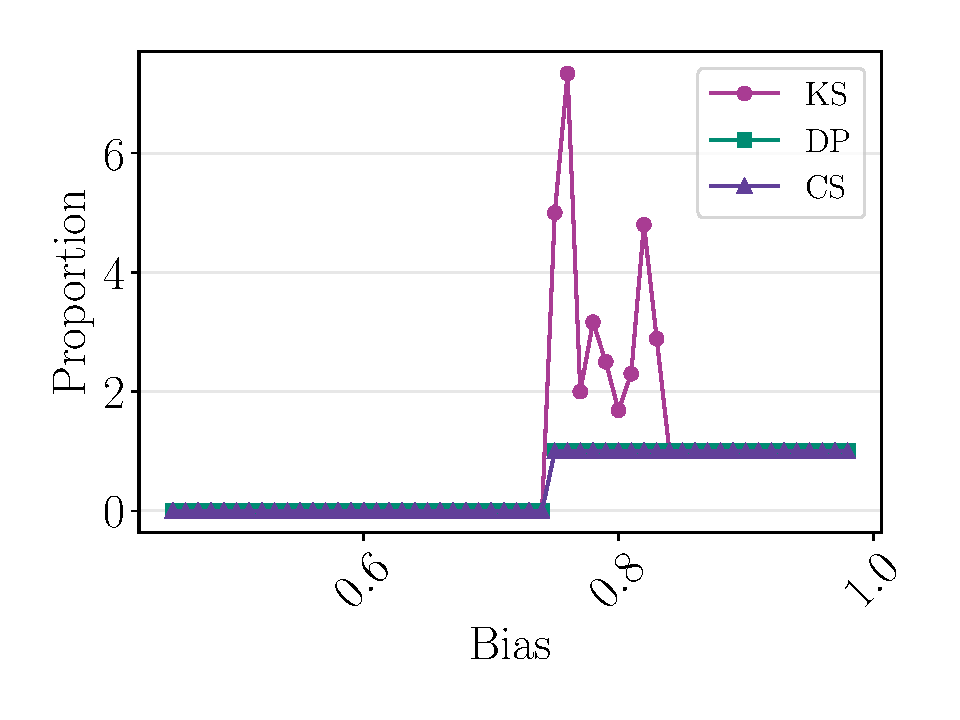
\includegraphics[width=\textwidth]{Figures/cyclic_proportion_Proportion.pdf}
		\caption{The proportion of cyclic profiles remaining, 0 indicating that no cyclic profiles were present after deliberation.}
		\label{fig:rep_cyclic}
	\end{minipage}\hfill
	\begin{minipage}{0.45\textwidth}
		\centering
		\vspace{-9pt}
		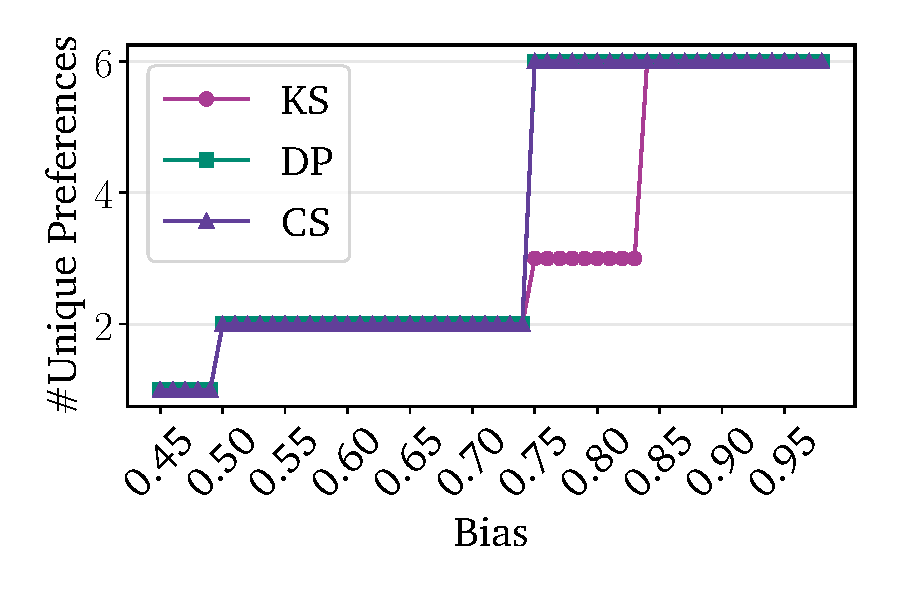
\includegraphics[width=\textwidth]{Figures/unique_Unique Preferences.pdf}
		\caption{Number of unique preferences at the final step of deliberation.}
		\label{fig:rep_count}
	\end{minipage}

	\vspace{1em}

	\begin{minipage}{0.45\textwidth}
		\centering
		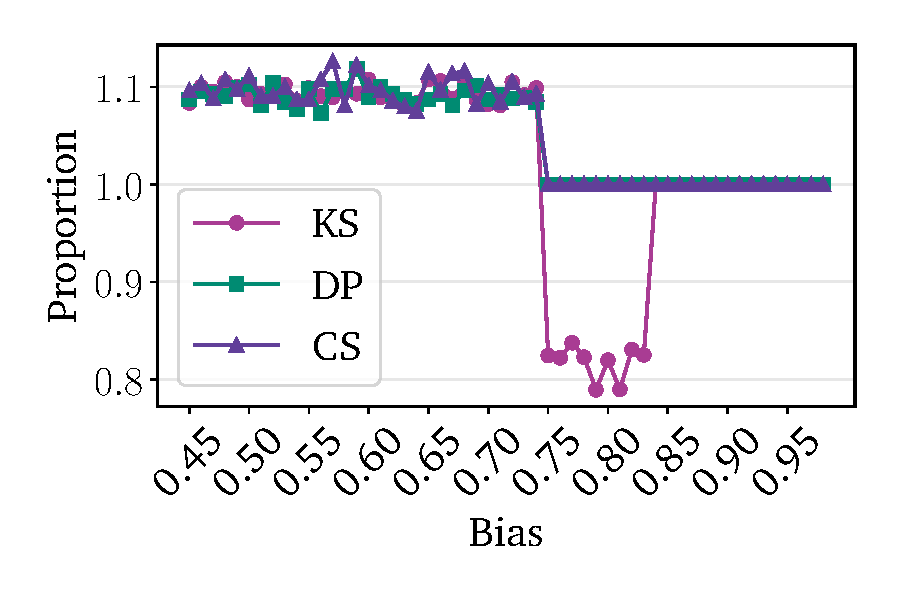
\includegraphics[width=\textwidth]{Figures/condorcet_proportion_Proportion.pdf}
		\caption{The proportion of Condorcet winners left after deliberation, value above one indicate Condorcet winners emerging during deliberation}
		\label{fig:rep_condorcet}
	\end{minipage}\hfill
	\begin{minipage}{0.45\textwidth}
		\centering
		\vspace{-9pt}
		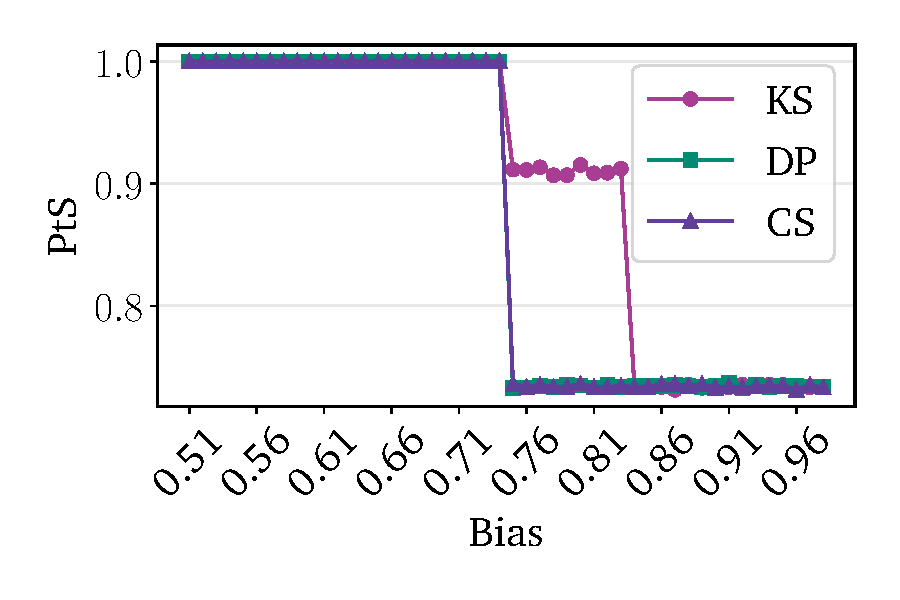
\includegraphics[width=\textwidth]{Figures/sp_proximity_PtS.pdf}
		\caption{Proximity to single-peakedness after deliberation. Proximity to single-peakedness as defined in \Cref{section:related_work}.}
		\label{fig:rep_single_peaked}
	\end{minipage}
\end{figure}
\newpage
\section{DeGroot Model} \label{degroot_results} \subsection{PBS Scores} We
first proceed with analyzing the performance of the DeGroot model on
substantive agreement. \Cref{fig:pbs} shows the PBS of both the
deliberation and control group, and the simulation results for both instances.
As mentioned in \Cref{sub:americainonroom}, the PBS (PBS) is the
average of the 26 most polarizing questions, where a low PBS corresponds to
more liberal answers, and high PBS indicates more conservative answers. As
expected the model performs poorly at predicting the control group, as there
was no significant change for control group members. Similar to the control
group, the starting  PBS of the participants is a strong indicator for
their  PBS. Therefore the model at t=0 is already reasonably aligned with
the final  PBS. We see that after the first time step the PBS scores get
predicted more accurately, after which the model starts making larger
prediction errors. This is because the model keeps averaging all opinions until
a steady state is reaches in which most voters hold non-extreme positions.
Whether this is positive depends on reality, as
\citet{elsterMARKETFORUMThree2002} remarked, if deliberation is able to reach
full consensus, the model might give a glimpse into how this works. If this is
not the case however, then the model is overly naive suggesting that people
come to hold a weighted average of all original opinions. The latter seems more
likely.


\begin{figure}[h]
	\begin{center}
		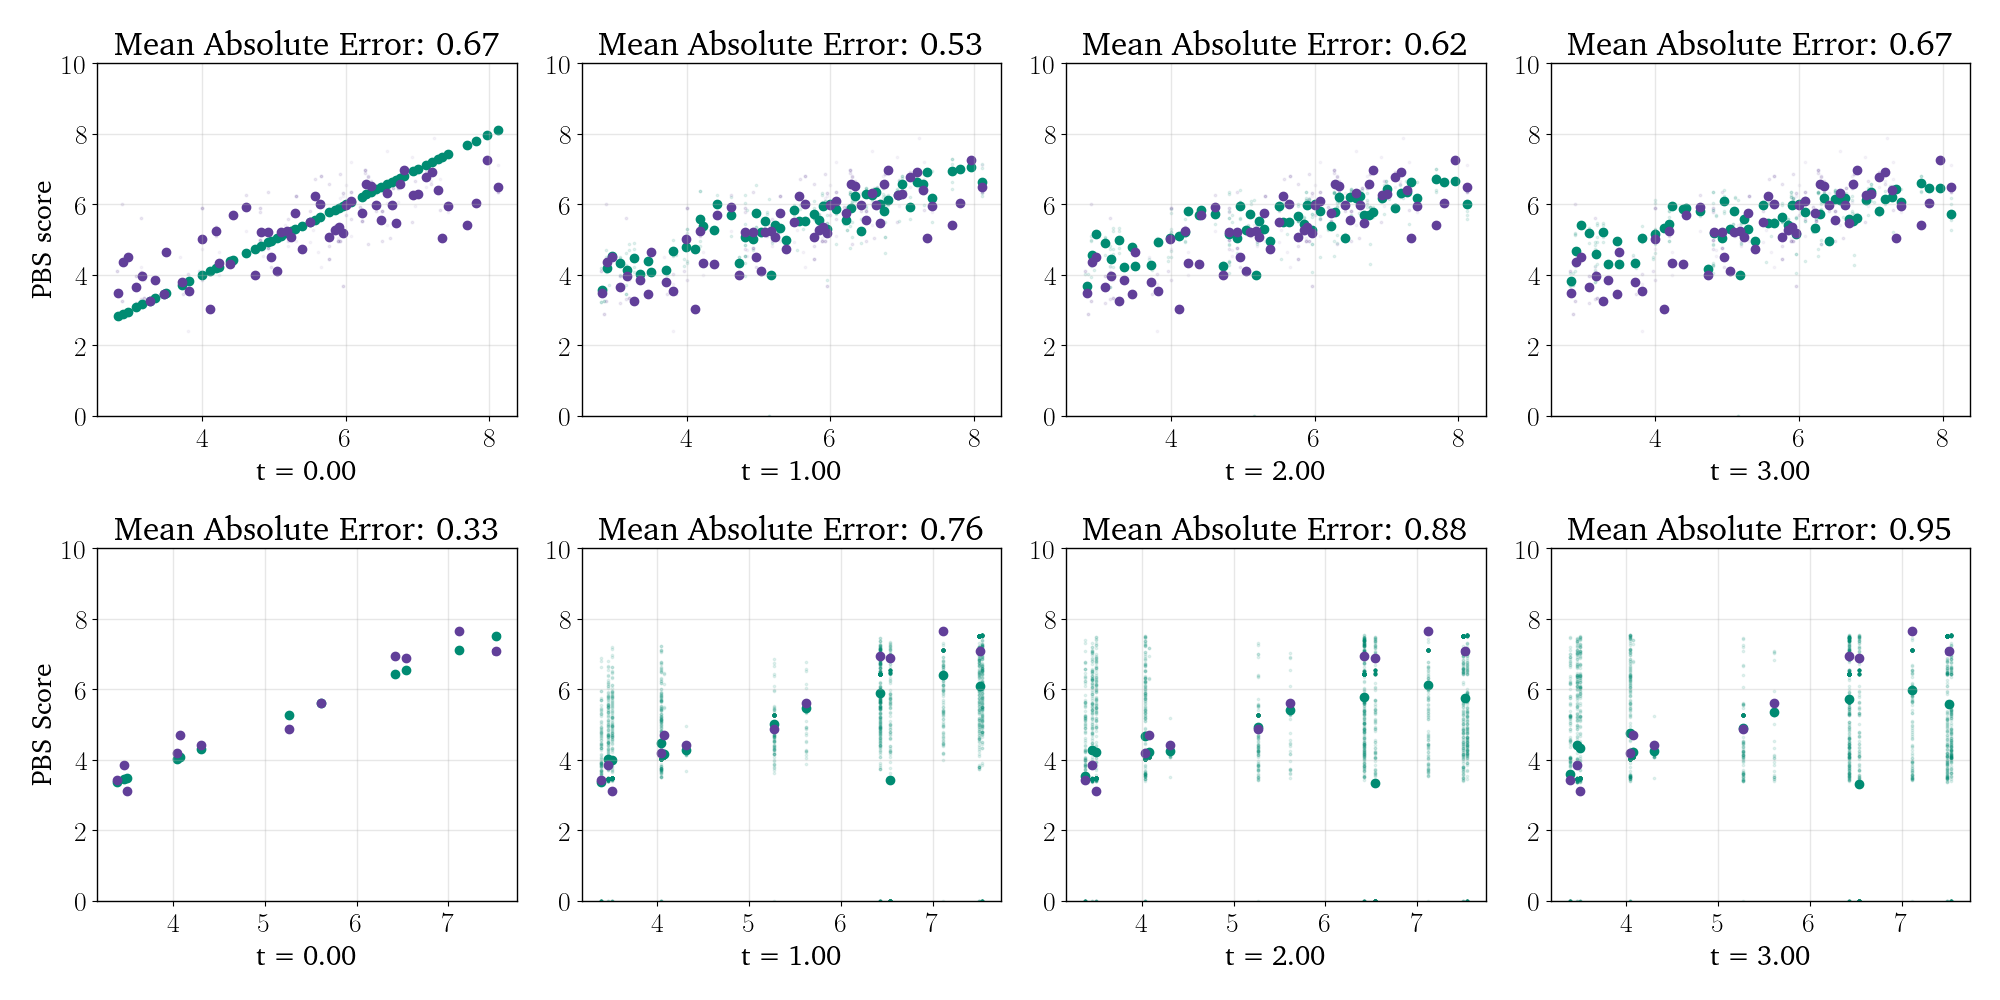
\includegraphics[width=0.95\textwidth]{Figures/pbs_scores.png}
	\end{center}
	\caption{ PBS, purple indicating the PBS score after deliberation in the original data, green indicates the results of the simulation in that time step.}\label{fig:pbs}
\end{figure}

\Cref{fig:delta_pbs} shows the change in  PBS for the deliberation group,
the original data shows most change happens in people with high  PBS,
getting lower PBS and thus becoming less extreme. The model does not capture
this effect, showing the most change for people with low initial  PBS in
later time steps. This might be because there is a correlation between PBS
score and knowledge. As shown by \citet{fishkinCanDeliberationHave2024}, most
extreme voters, in terms of PBS, seemed to also be the most knowledgeable, if
this was skewed towards voters with high PBS, then these voters would have more
effect on people's opinions in this model when using knowledge-based trust.
Looking at the binned errors in \Cref{fig:binned_errors}, we see that the model
performs better when we do not include knowledge, further indicating that
knowledge is a poor predictor of trust, or persuasiveness. Of course this claim
might be weakened by noting that knowledge in this case is measured by
questions regarding the current state of the America government, such as know
which party currently has a majority in the senate. Thus, this specific
knowledge might be insufficient to predict someone's persuasiveness on the
topic of immigration for example.


\begin{figure}[h]
	\begin{center}
		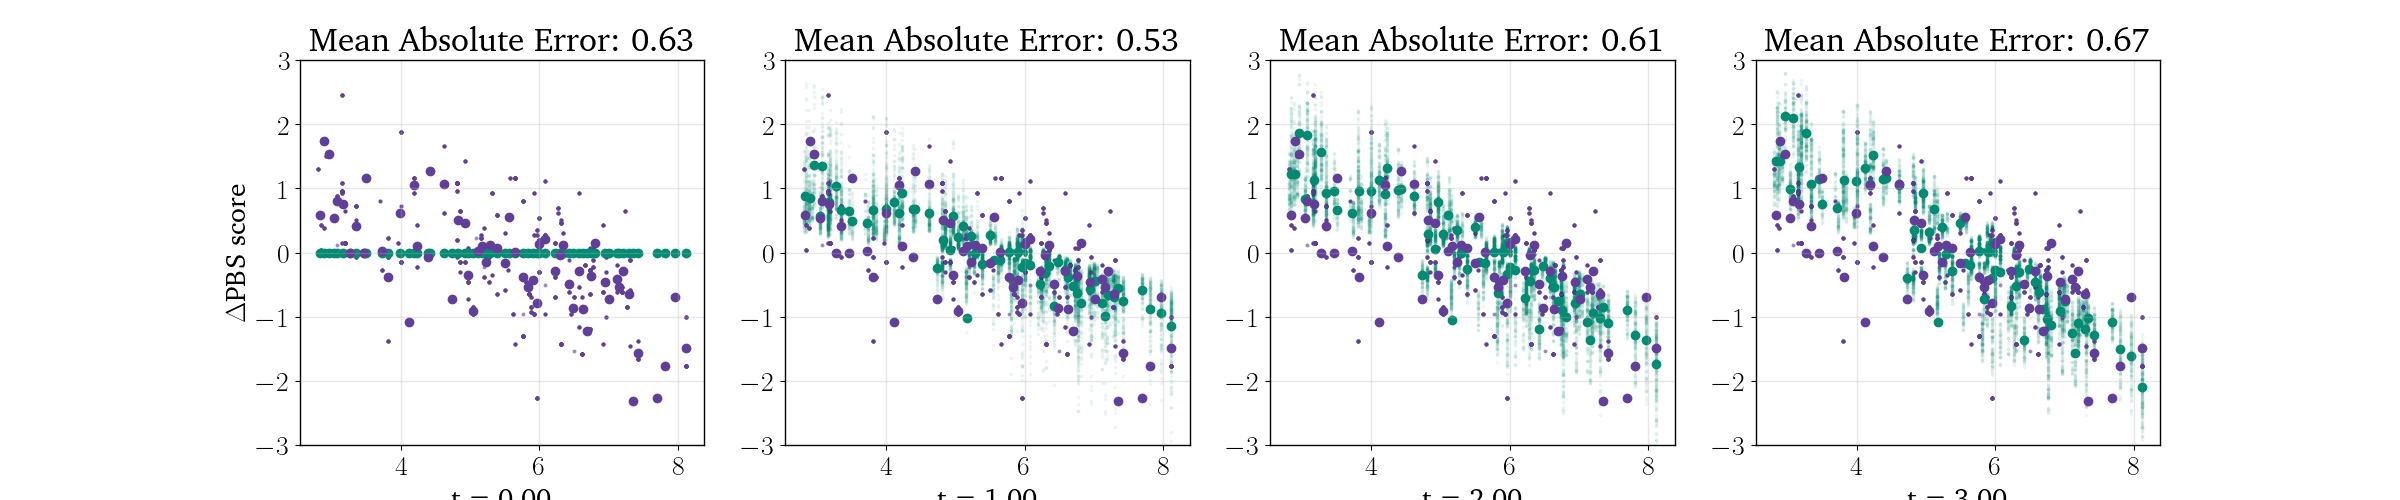
\includegraphics[width=\textwidth]{Figures/change_pbs_scores.png}
	\end{center}
	\caption{Change in  PBS, relative to the original, pre deliberation, measurement. The control is  omitted as there was no significant change.}\label{fig:delta_pbs}
\end{figure}


We note that this slight positive results appear only when the voters are
grouped by their original PBS, thereby giving the model reasonable predictive
power over a population of voters. We note that this hold even for different
sizes of bins. \Cref{fig:binned_errors} shows the progression of errors over
time when the error is calculated on a per-individual basis, and we find the
model consistently does worse than predicting someone to not change their
opinion, which is what t=0 indicates.

\begin{figure}[h]
	\begin{center}
		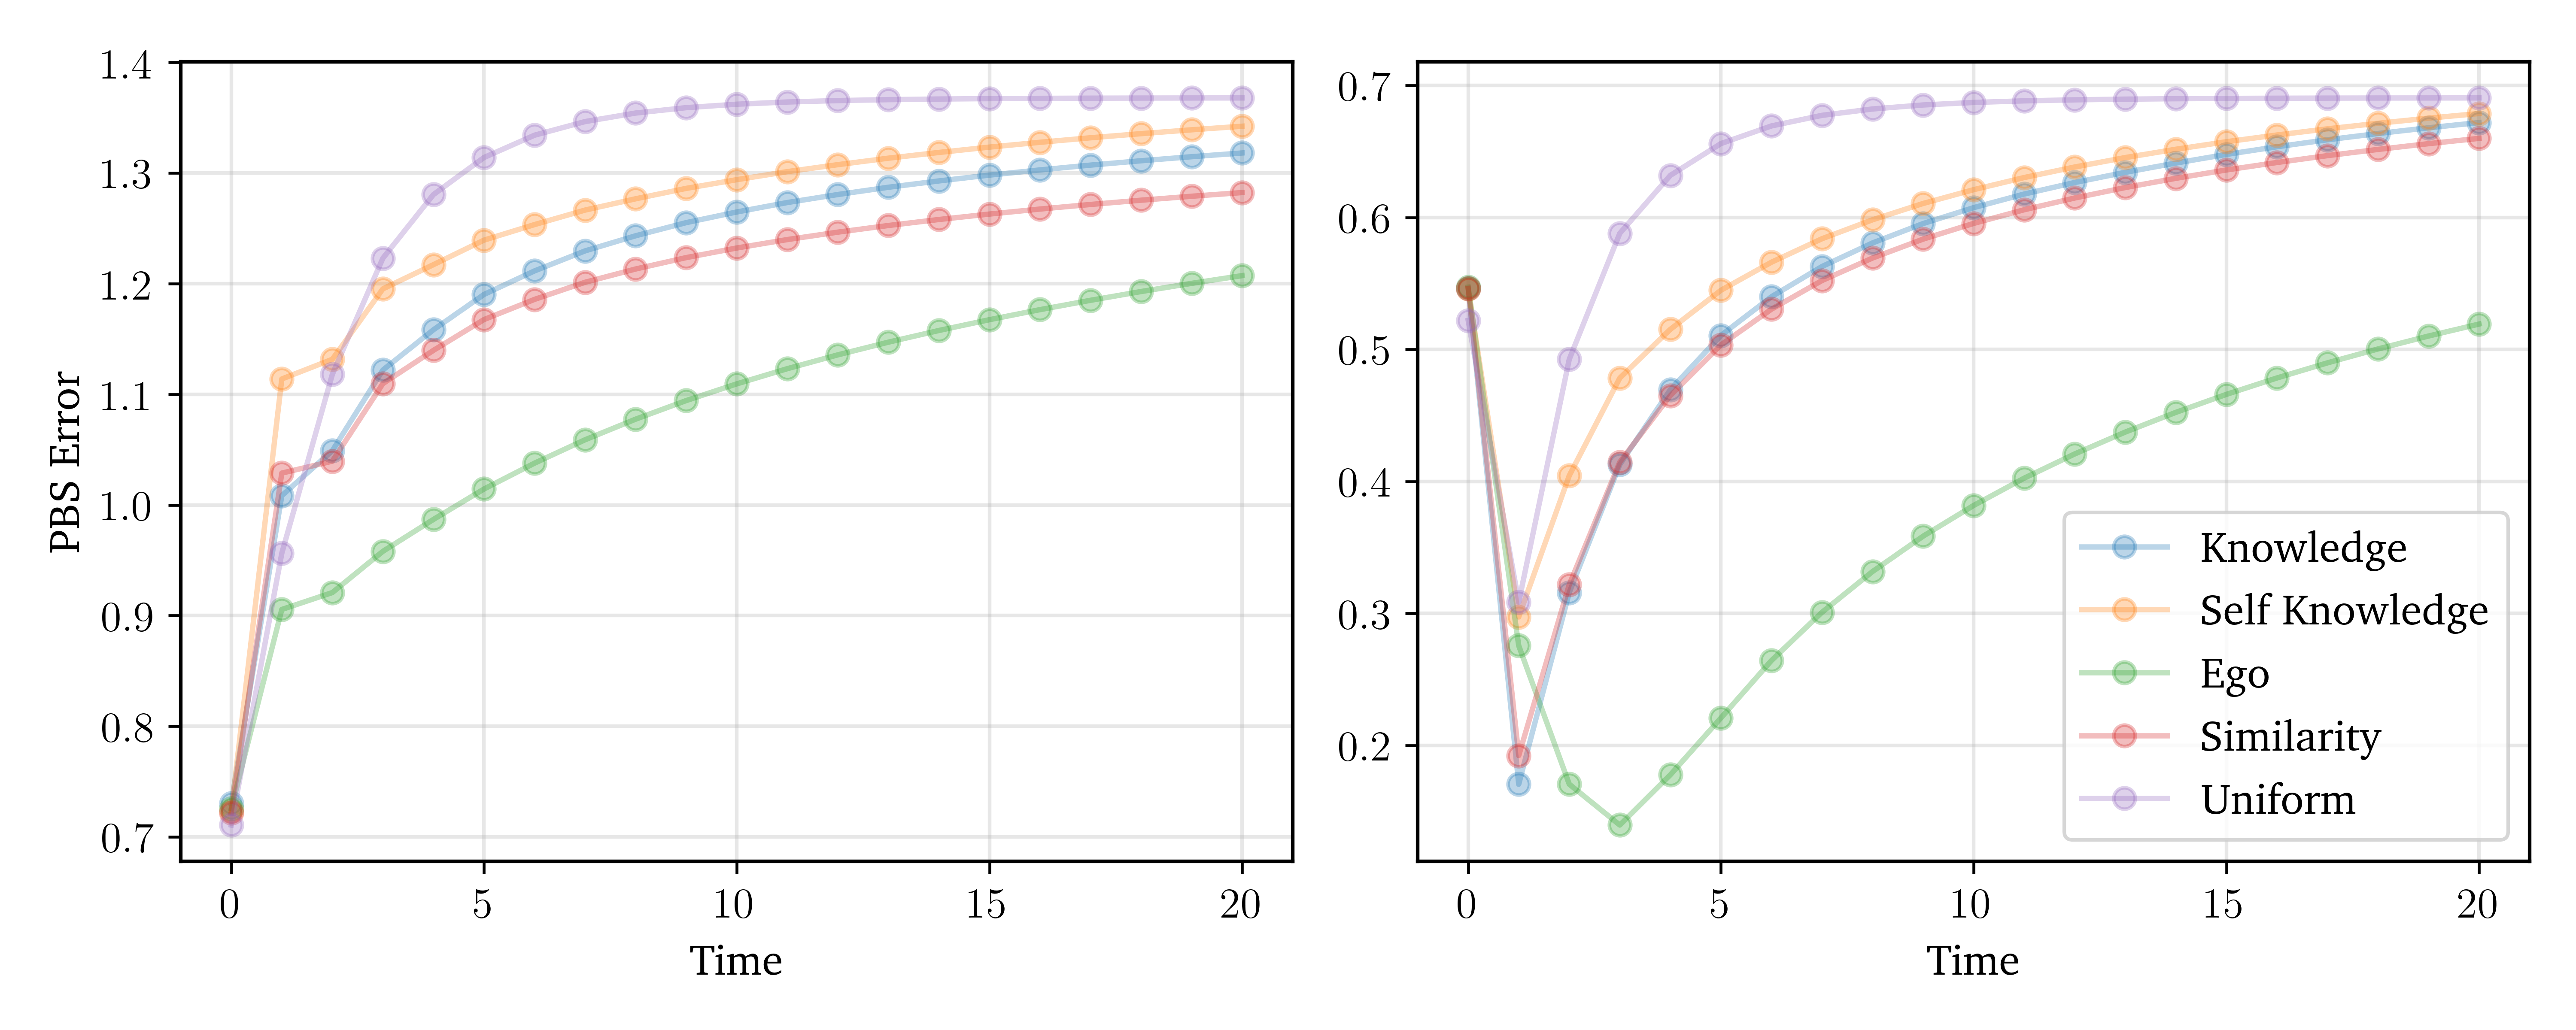
\includegraphics[width=0.95\textwidth]{Figures/errors_binned.png}
	\end{center}
	\caption{Prediction error of the model as a function of time, binned relative to the original  PBS.}\label{fig:binned_errors}
\end{figure}


\begin{figure}[h]
	\centering

	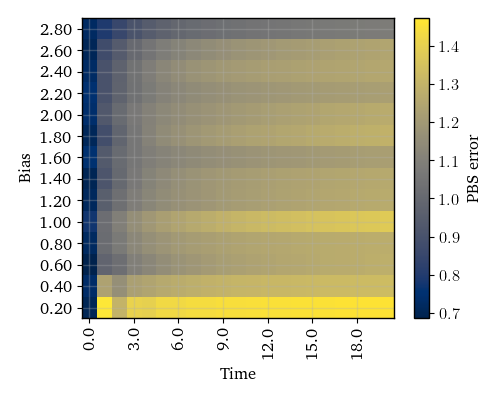
\includegraphics[width=0.6\textwidth]{Figures/bias_time_imshow.png}
	\hspace{1em}
	\caption{PBS Errors as a function of bias and time. bias acts as a damper, when bias is higher the model take longer to over estimate the change in opinion.}
	\label{fig:bias_slowdown}
\end{figure}

\Cref{fig:bias_slowdown} shows the relation between the bias factor and the PB
score, showing that the bias does not improve the models predictive power. As
one might expect a bias is ``slowing down'' the model. Because of this the
model is slower to diverge away from the true opinions.

Finally, \Cref{tab:anova_trust} shows the results of an ANOVA analysis over the
four different methods. The knowledge method is the only non-significant
method, meaning that including knowledge in your model does not significantly
impact the simulation results and therefore it has no effect on the model
error. All other methods do significantly affect the outcome of the model. We
find that the model has the lowest error when we include self-ego and
similarity, but exclude self-knowledge.


\begin{table}
	\caption{F-statistics for the different trust matrix generators.}\label{tab:anova_trust}
	\begin{center}
		\begin{tabular}[c]{lcr}
			\toprule
			Method & F-statistic& p-value \\
			\hline
			Knowledge & 0.3 & 0.57 \\
			Ego & 48.4& $<0.01$ \\
			Similarity & 21.7& $< 0.01$ \\
			Self-Knowledge & 163.6& $ <0.01$ \\
			
			\bottomrule
		\end{tabular}
	\end{center}
\end{table}

\subsection{Convergence}

From \Cref{theory}, we have seen that in the limit some matrices are
convergent, while some are not, in particular if the matrix is aperiodic, this
it is convergent. As we model the deliberation group as having fully connected
matrices, the matrices are aperiodic, and thus convergent. We look at the
distance between the estimated support matrix, and the true support matrix, to
get a sense of the rate of convergence. The distance is defined as the 
$\ell_1$ norm.

\begin{figure}[h]
	\begin{center}
		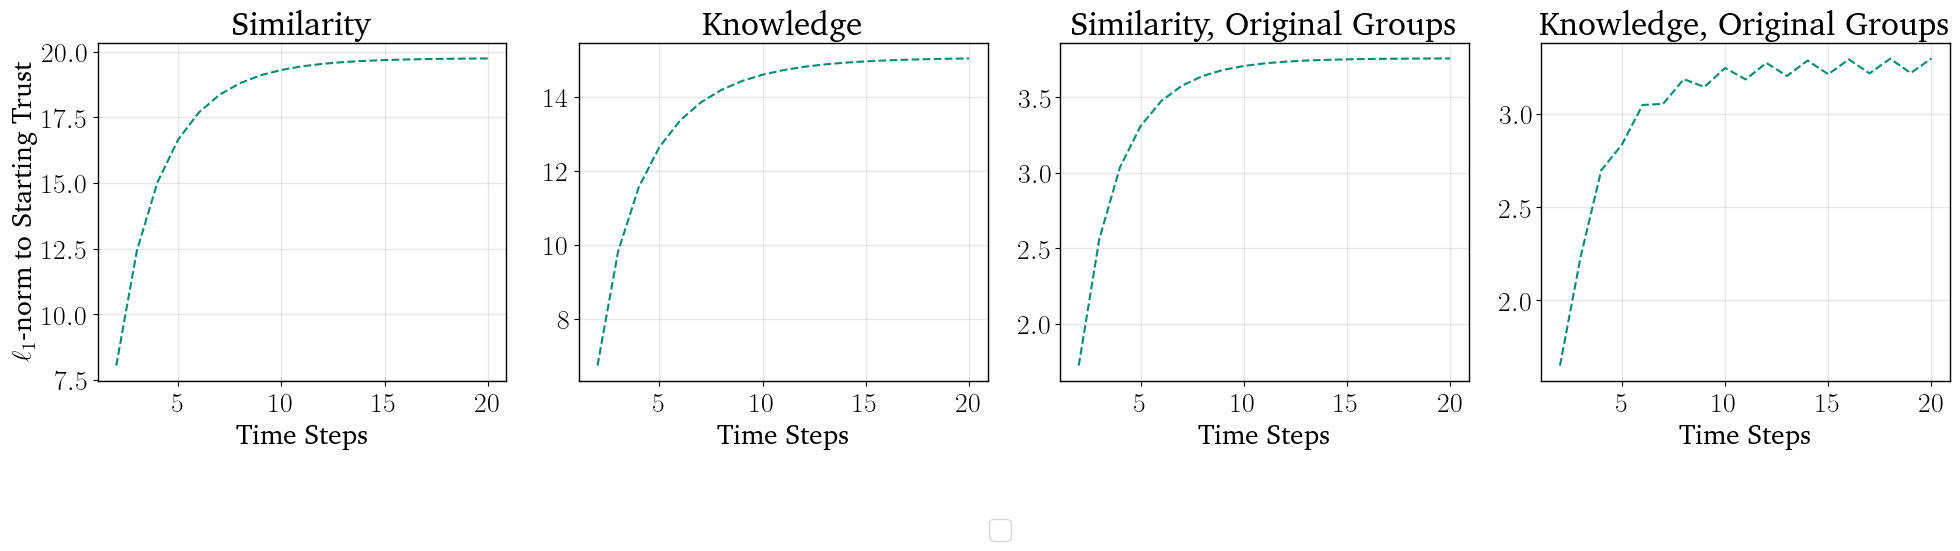
\includegraphics[width=0.95\textwidth]{Figures/convergence_groups.png}
	\end{center}
	\caption{Convergence of trust matrices, as measured by the $\ell_1$-norm between the trust matrix at the start and  trust matrix at the current time step
		t}\label{fig:convergence_big}
\end{figure}




% We now proceed to look at distance to single-peaked profiles, look at both
% voter removal and candidate removal. We show that for optimal bias, as
% deliberation progresses we see an increase in the proximity to single
% peakedness.

\section{Sensitivity Analysis} We perform sensitivity analysis on the
prediction error of our model on the PBS. For this we do not use the original
groups, instead reassigning voters to random groups of constant size.
\Cref{fig:sensitivty_pbs} shows the sensitivity indices, the \textit{number of voters}
is clearly the biggest factor in the variance of the model. As expected the
\textit{bias} does not contribute to the variance in the model. \textit{Knowledge} informed bias
and\textit{ similarity} informed \textit{bias} both are significantly impacting the variance of
the model. The second order indices show \textit{number of voters} interacts with
self-knowledge and\textit{ similarity}, contributing a large portion of their explained
total variance induced by the \textit{number of voters}. Similarly,\textit{ knowledge}-based
trust and\textit{ similarity}-based trust both have most of their explained variance in
their interactions, since their first order sensitivity is statistically
significant, but low in magnitude.



\begin{figure}[h]
	\begin{center}
		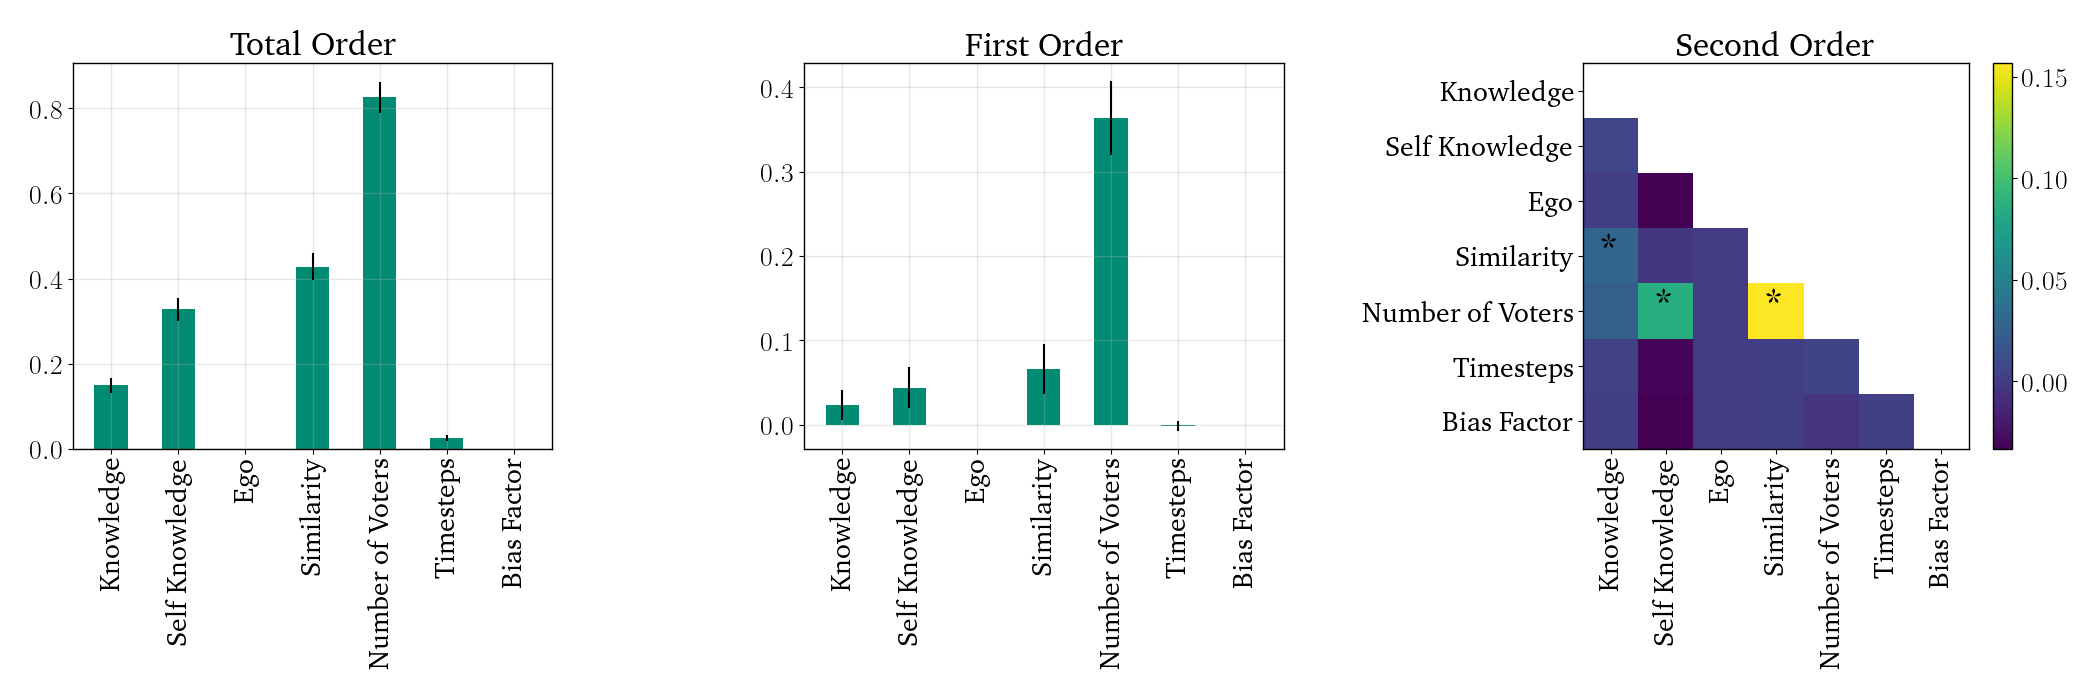
\includegraphics[width=0.95\textwidth]{Figures/senstivity_analysis.png}
	\end{center}
	\caption{First, Second and Total sensitivity indices on the PBS prediction error. The stars in the heat map for the Second order sensitivity indices indicate significant interactions. }\label{fig:sensitivty_pbs}
\end{figure}


\section{Elections}

\begin{figure}[htbp]
	\centering
	\begin{minipage}{0.45\textwidth}
		\centering
		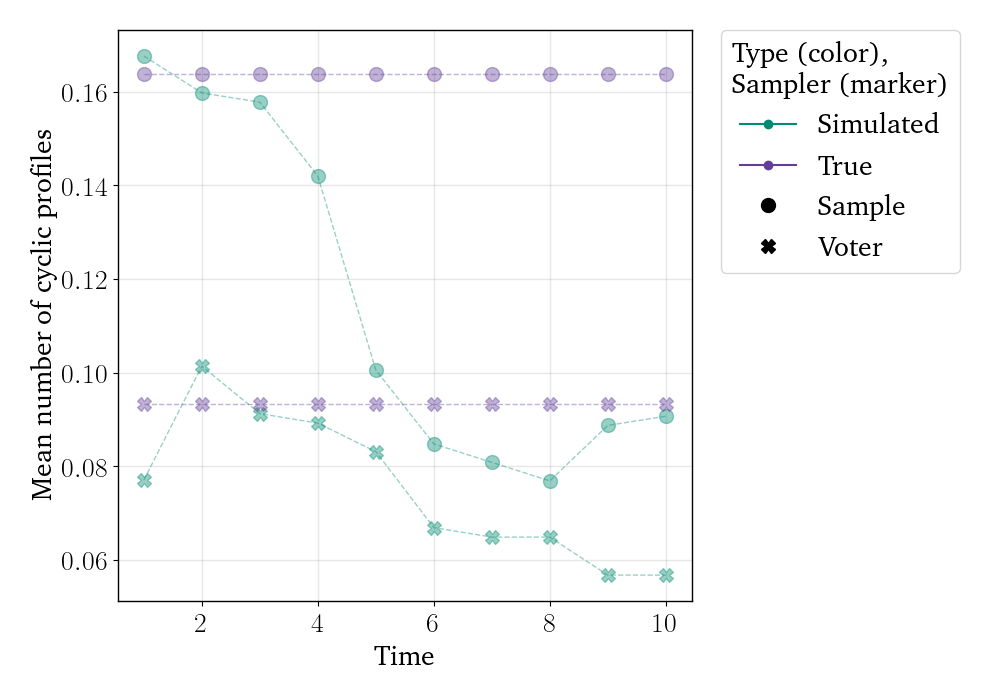
\includegraphics[width=\textwidth]{Figures/delib_Mean Number of Cyclic Profiles.png}
		\caption{The proportion of cyclic profiles remaining, 0 indicating that no cyclic profiles were present after deliberation.}
		\label{fig:degroot_cyclic}
	\end{minipage}\hfill
	\begin{minipage}{0.45\textwidth}
		\centering
		\vspace{-9pt}
		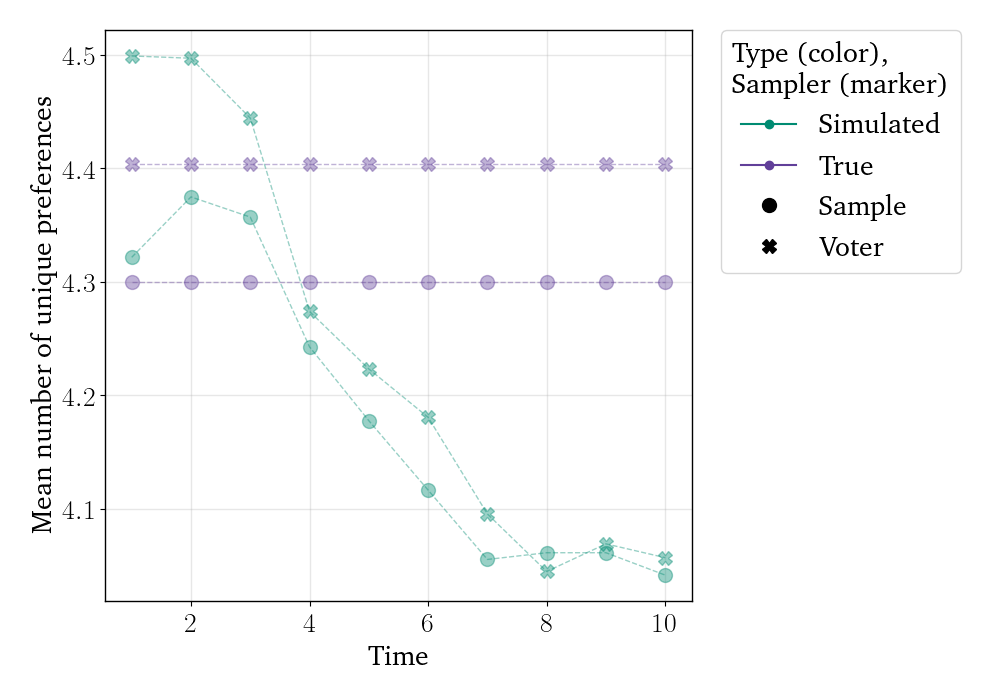
\includegraphics[width=\textwidth]{Figures/delib_Mean number of Unique Preferences.png}
		\caption{Number of unique preferences at the final step of deliberation.}
		\label{fig:degroot_count}
	\end{minipage}

	\vspace{1em}

	\begin{minipage}{0.45\textwidth}
		\centering
		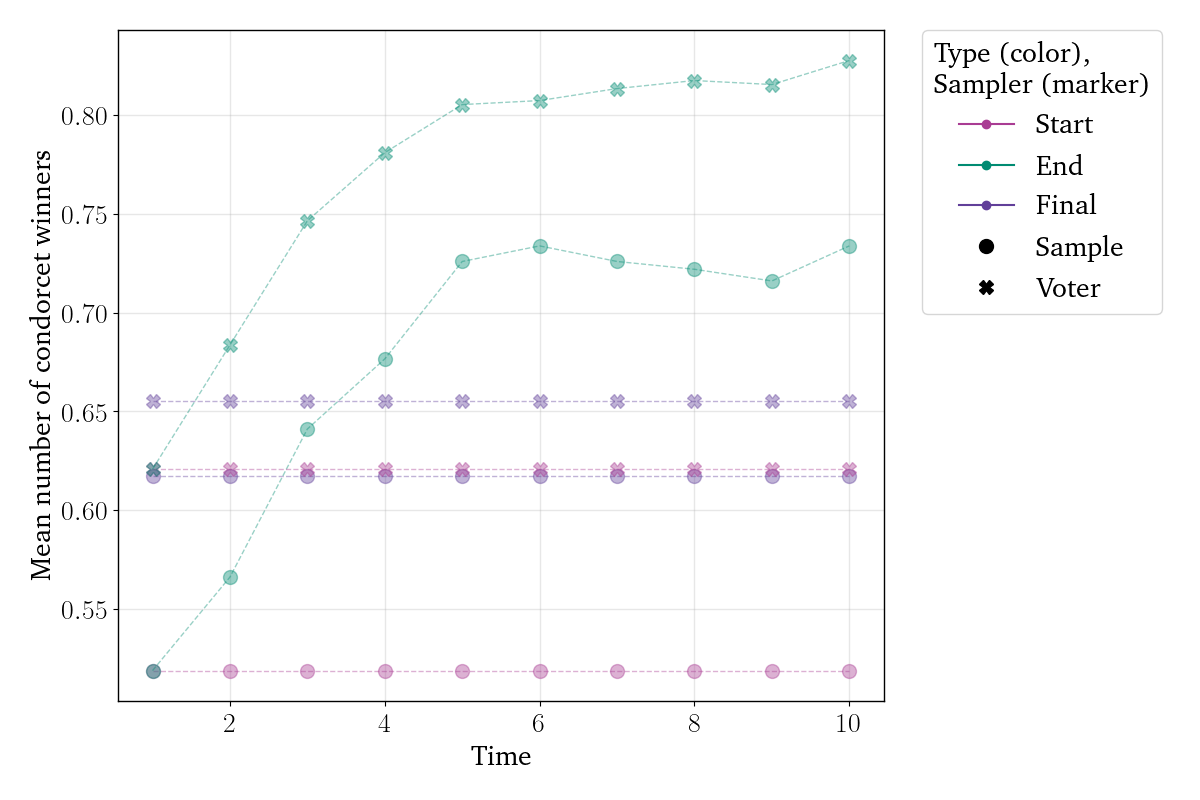
\includegraphics[width=\textwidth]{Figures/delib_Mean number of Condorcet winners.png}
		\caption{The proportion of Condorcet winners left after deliberation, value above one indicate Condorcet winners emerging during deliberation}
		\label{fig:degroot_condorcet}
	\end{minipage}\hfill
	\begin{minipage}{0.45\textwidth}
		\centering
		\vspace{-9pt}
		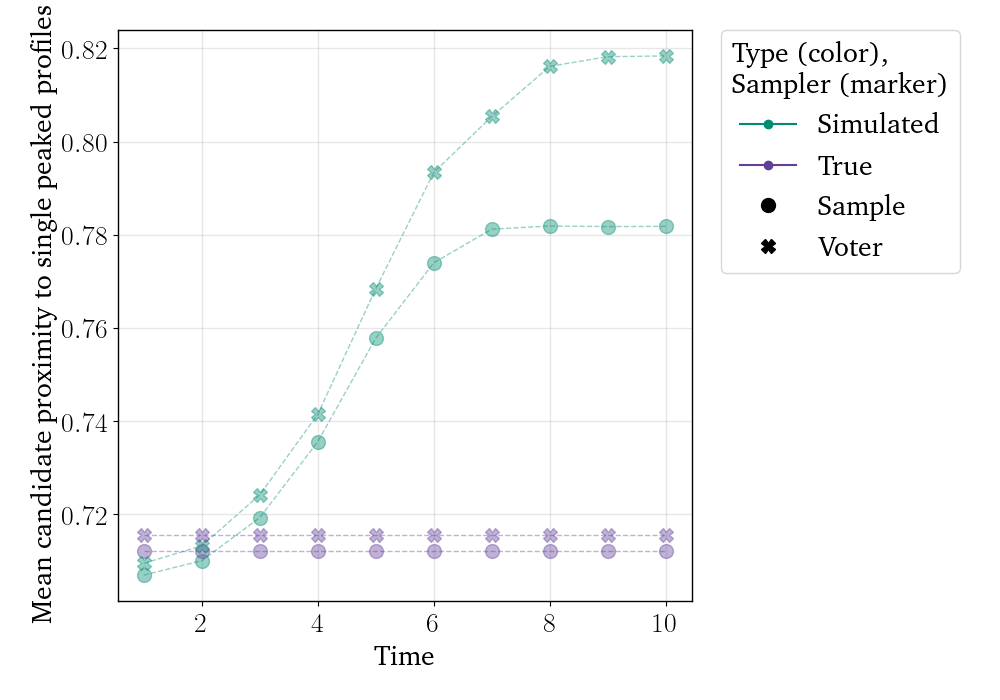
\includegraphics[width=\textwidth]{Figures/delib_Mean candidate proximity to single peaked Profiles.png}
		\caption{Proximity to single-peakedness after deliberation. Proximity to single-peakedness as defined in \Cref{section:related_work}.}
		\label{fig:degroot_single_peaked}
	\end{minipage}
\end{figure}


Firstly, looking at the different voter generation mechanisms, we find that in
general they do not affect the metrics much. The metric for which this is not
true is that of the fraction of elections with a Condorcet winner. Though
slightly unintuitive, we suspect the reason why a single voter's opinion is
more likely to result in a Condorcet winner than the average of 10 voters is
that the true opinions before deliberation were more polarized. As a result,
having multiple ``average'' candidates results in little difference between
them, while an individual voter is more likely to fall close to a large camp of
voters, and thus become a Condorcet winner through being closer to a majority
of voters.

Looking at the metrics evaluated on the model, we see similar results as with
the analysis for substantive agreement. At first the simulation starts far from
the metrics from the true score, then it moves towards it and overshoots it
until it starts to converge. Interestingly, for these metrics, the model does require more steps to converge to the same values as the true data.

\textcolor{gray}{This last analysis is very short and needs work}
